\documentclass[rapport.tex]{subfiles}

\begin{document}
\section{Kravspecifikation}
\label{sec:kravspec}

	\subsection{Problemstillinger}
	Der ønskes udviklet et system som kan indsamle videodata fra et kamera og derefter anvende dataen til
	at bestemme hvor en forsøgsperson kigger hen på en specifik skærm. Systemet skal derudover videregive
	denne information til brugeren via koordinater samt en graf der repræsenterer den skærm forsøgspersonen
	ser på.
	\\
	\indent
	Før dataopsamling skal en indledende kalibrering af systemet gennemføres. Dette gøres ved at et gitter med
	specifikke punkter indlæses på forsøgspersonsskærmen. Derefter bedes forsøgspersonen fiksere på specifikke punkter
	på skærmen, og sammenhængen imellem de målte punkter og de kendte punkter kan anvendes til at finde en
	homografisk mapning. Efter denne kalibrering kan systemet anvendes.
	\\
	\indent
	Systemet udvikles med henblik på en standard anvendelsesmåde, med mulighed for brugerdefinerede anvendelsesmåder. 
	Standardanvendelsen omhandler at vælge en sti og et filnavn, hvorefter dataopsamling umiddelbart begynder.
	Under dataopsamlingen vil gazevectoren løbende blive præsenteret for brugeren på brugerskærmen. Når brugeren er 
	færdig kan opsamlingen stoppes, og dataopsamlingen gemmes i den tidligere valgte fil. Bemærk at den algoritme
	der anvendes til behandling af data her er forudbestemt.
	\\
	(Hvis brugeren ønsker at bruge en anden algoritme kan denne indlæses. Den kan også indskrives direkte i
	GUI'en, og derefter gemmes. Formålet med dette er at kunne indrette systemet efter specifikke behov, og
	hurtigt indhente de opsætninger til fremtidig brug. Eventuelt kan andre variabler indtastes ved systemstart) 
	\\
	\indent
	I de følgende afsnit fremgår det hvorledes det udviklede system indgår i det samlede system.
	
	
	\subsection{Funktionelle krav}
	Følgende funktionelle krav for systemet er blevet stillet: \\
	\begin{enumerate}
		\item 
		\textbf{Real-time eye-tracking}: Systemet skal kunne foretage real-time eye-tracking.
		\item 
		\textbf{Kalibrering}: Før måling skal programmet kunne kalibreres.
		\item
		\textbf{Output}: Resultater af måling skal ende i en log-fil tilgængelig til brugeren.
		\item
		\textbf{Modularisering}: Det skal være muligt for bruger at ændre/erstatte algoritmen.
		\item
		\textbf{Brugertilgang}: Ved hjælp af use case teknikken vil en yderlige række krav blive stillet. Disse vil lægge grundlag for bruger-program-interaktioner. Use-case-kravene er opstillet i afsnit \ref{usec}.  
	\end{enumerate}
	
	\subsubsection{Real-time eye-tracking}
	Systemet skal kunne foretage real-time eye-tracking ved hjælp af en implementeret udgave af Starburst-algoritmen som givet af Siboska og OpenEyes.
	\subsubsection{Kalibrering}
	Specifikke ukendte variabler skal kunne kalibreres ved hjælp af interpolation. Herved skal programmet kunne tilpasses testpersonens fysiske forhold til kameraet. 
	\begin{figure}[h]
		\centering
		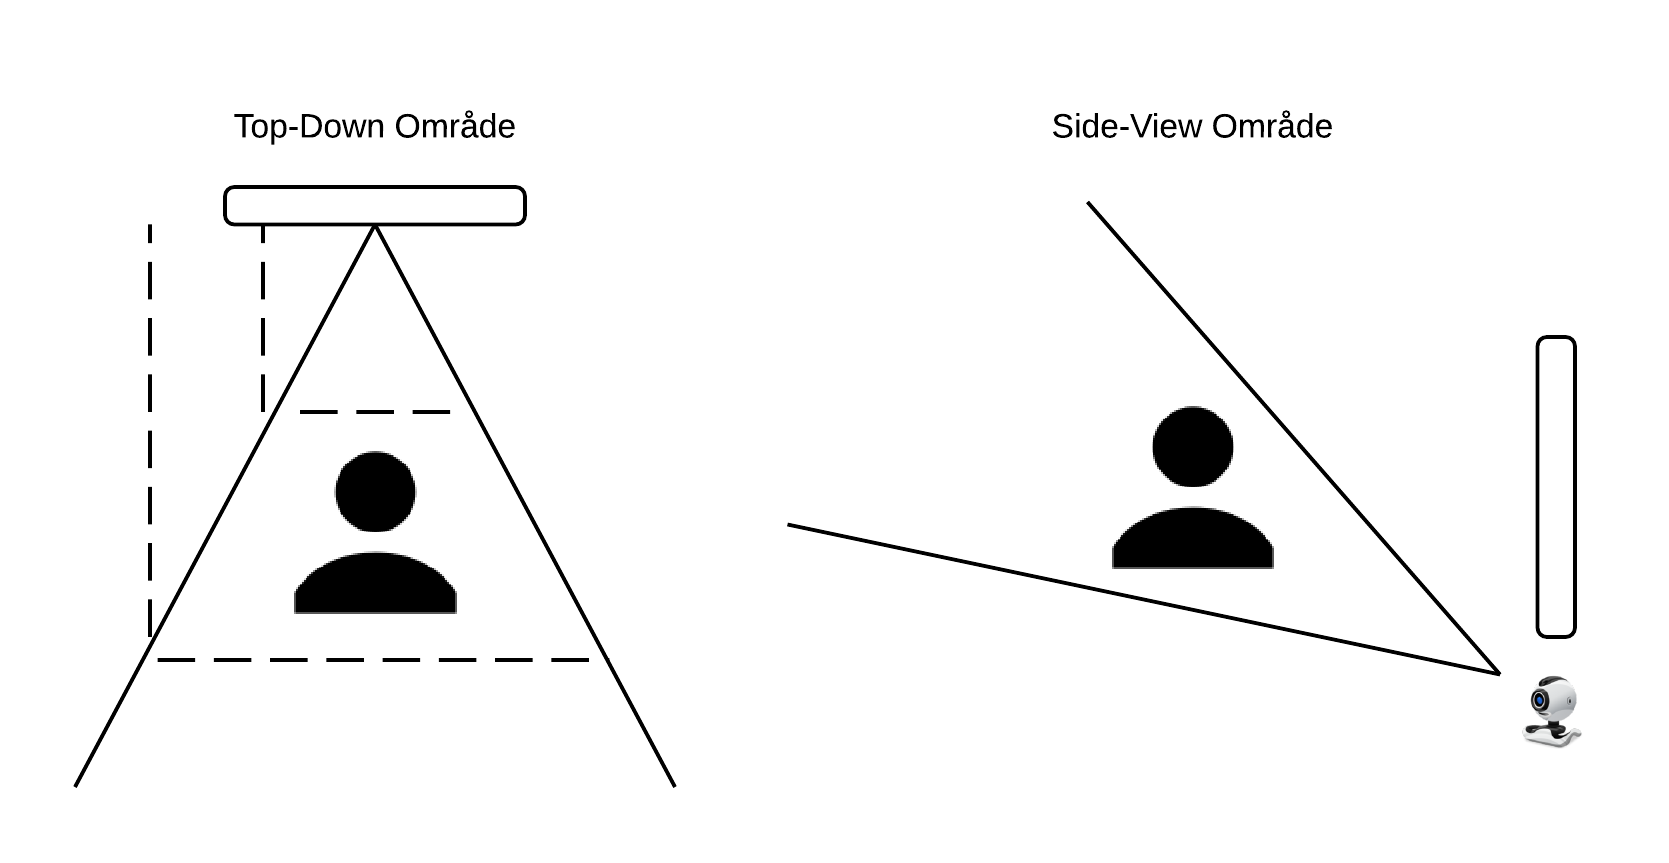
\includegraphics[width=0.7\linewidth]{../Kamera-testperson}
		\caption{Kameraets position i forhold til testperson}
		\label{fig:Camposition}
	\end{figure}
	
	
	Derudover skal programmet kunne kalibreres således at der kan findes tærskler (threshold-values) for trigger-niveauet: En værdi når trigger-niveauet går højt, og en værdi når trigger-niveauet går lavt.
	
	\begin{figure}[H]
		\centering
		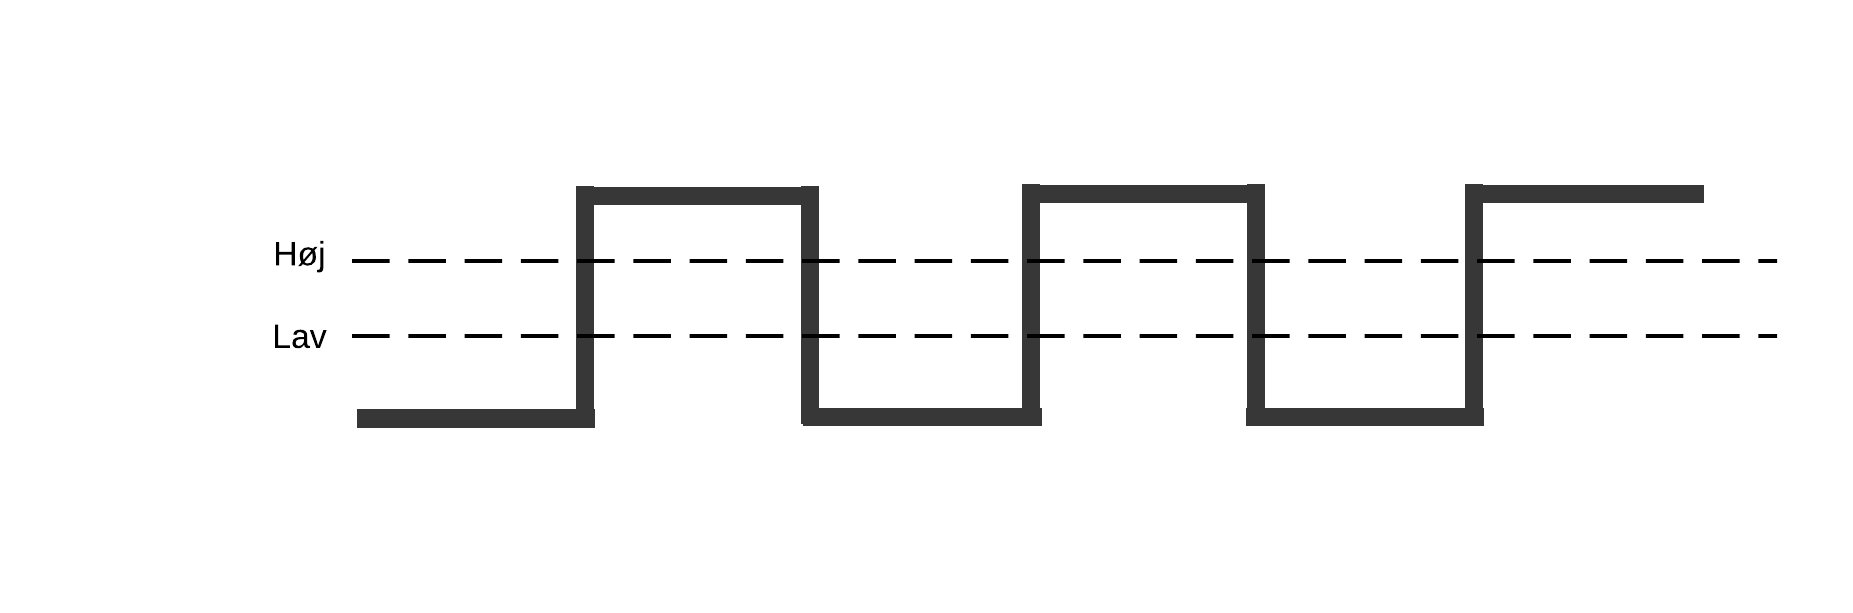
\includegraphics[width=0.7\linewidth]{../Trigger-threshold}
		\caption{Eksempel på tærskelværdier for trigger-signalet}
		\label{fig:Trigger-threshold}
	\end{figure}
	
	
	
	\subsubsection{Output}
	\label{sec:output}
	For hver igangsat session skal programmet generere en log-fil med følgende data:
	\indent \begin{itemize}
		
		\item 	Kommasepareret målingsdata med følgende format: \\
		\textit{timestamp, x-koordinat, y-koordinat, trigger, fejlmeddelelse}
	\end{itemize}
	
	\subsubsection{Modularisering}
	Systemet skal være modulariseret, således at bruger kan foretage ændringer i algoritmen, eller tilføje en hel ny algoritme. Det er derfor nødvendigt med en opdeling af programmet, samt klare regler for input-argumenter og output-værdier i forhold til algoritme-delen. 
	Dette system skal implementeres med Starburst-algoritmen som udgangspunkt.
	
	\subsubsection{Use-cases}	
	\label{usec}
	\begin{enumerate}
		\item Opret session: \\Opretter en session i en fil-sti med nødvendige data-filer. 
		\item Kalibrering: \\Initierer en række kalibreringer før brug. 
		\item Start måling: \\Igangsætter måling.
		\item Stop måling: \\Afslutter måling.
		\item Gem indstillinger: \\Gemmer en fil med brugerens nuværende indstillinger.
		\item Indlæs indstillinger: \\Indlæser indstillinger fra gemt fil.
		\item Indlæs rå data: \\Indlæser rå data fra tidligere session. 
	\end{enumerate}
	\subsection{Ikke funktionelle krav}
	Real-time eye-tracking systemet skal leve op til en række ikke funktionelle krav. Disse krav skal garantere et robust system, der med en hvis præcision skal kunne levere de ønskede data.\\
	\begin{itemize}
		\item 
		\textbf{Fejlmargin}: Systemet skal kunne angive XY-koordinater for øjets fokuspunkt. Disse koordinater må have en afvigelse på <2\degree \cite{FairchildInSiboska}.
		\item 
		\textbf{Real-time}: Systemet skal kunne angive XY-koordinater med en frekvens bestemt af kameraets frame-rate. 
		\item
		\textbf{Kamera}: Skal kunne levere video-data real-time til en computer. Systemet bliver udviklet til kamera af typen Basler
		ACA640-100gc GigE med opløsningen 658 x 492 pixels og maksimum framerate på 100Hz.
		\item Følgende krav er ikke krav til systemet, men krav til testpersonens fysiske forhold til kameraet. Dette er relevant når der foretages eye-tracking. \\
		\textbf{Afstand og skærm}: Systemet bliver udviklet med en afstand fra kamera til testperson på 60cm. 
		På samme afstand fra testpersonen er der placeret en skærm. Denne skærm har størrelsen 26 tommer.
	\end{itemize}
	
	Typen af kamera og afstand til testperson kommer fra tidligere forsøg \cite{Siboska}.
	\subsection{Performance-evaluering}
	Systemet kan efter implementering og test evalueres efter performance. Følgende punkter ønskes evalueret:
	\begin{itemize}
		\item \textbf{Miljø}: Algoritmens evne til at til at tilpasse sig forskellige afstande til forsøgspersonen, forsøgspersonens bevægelser, samt forskellige lysstyrker. 
		\item \textbf{Robusthed}: Systemets evne til at håndtere fejl under måling. 
		\item \textbf{Brugervenlighed}: Systemets evne til at håndtere fejl i det grafiske bruger-interface. Simplicitet af det grafiske bruger-interface.  
	\end{itemize}
	
	\subsection{Diskussion}
	De formulerede krav medfører en afgrænsning af projektet, og ligger basis for arbejdet med v-modellen. 
	
		
\end{document}